
%\documentclass[mathserif]{beamer}
\documentclass[handout]{beamer}
%\usetheme{Goettingen}
%\usetheme{Warsaw}
\usetheme{Singapore}



%\usetheme{Frankfurt}
%\usetheme{Copenhagen}
%\usetheme{Szeged}
%\usetheme{Montpellier}
%\usetheme{CambridgeUS}
%\usecolortheme{}
%\setbeamercovered{transparent}
\usepackage[english, activeacute]{babel}
\usepackage[utf8]{inputenc}
\usepackage{amsmath, amssymb}
\usepackage{dsfont}
\usepackage{graphics}
\usepackage{cases}
\usepackage{graphicx}
\usepackage{pgf}
\usepackage{epsfig}
\usepackage{amssymb}
\usepackage{multirow}	
\usepackage{amstext}
\usepackage[ruled,vlined,lined]{algorithm2e}
\usepackage{amsmath}
\usepackage{epic}
\usepackage{epsfig}
\usepackage{fontenc}
\usepackage{framed,color}
\usepackage{palatino, url, multicol}
%\algsetup{indent=2em}
\newcommand{\factorial}{\ensuremath{\mbox{\sc Factorial}}}
\newcommand{\BIGOP}[1]{\mathop{\mathchoice%
{\raise-0.22em\hbox{\huge $#1$}}%
{\raise-0.05em\hbox{\Large $#1$}}{\hbox{\large $#1$}}{#1}}}
\newcommand{\bigtimes}{\BIGOP{\times}}
\vspace{-0.5cm}
\title{Natural Language Processing \\ Linear Models}
\vspace{-0.5cm}
\author[Felipe Bravo Márquez]{\footnotesize
%\author{\footnotesize  
 \textcolor[rgb]{0.00,0.00,1.00}{Felipe Bravo-Marquez}} 
  
 

\date{\today}

\begin{document}
\begin{frame}
\titlepage


\end{frame}



\begin{frame}{Supervised Learning}
\begin{scriptsize}
\begin{itemize}
\item The essence of supervised machine learning is the creation of mechanisms that can look at examples and produce generalizations. \cite{goldberg2017neural}
\item We design an algorithm whose input is a set of labeled examples, and
its output is a function (or a program) that receives an instance and produces the desired label.
\item Example: if the task is to distinguish from spam and not-spam email, the labeled examples are emails labeled as spam and emails labeled as not-spam.
\item It is expected that the resulting function will produce correct label
predictions also for instances it has not seen during training.
\item This approach differs from designing an algorithm to perform the task (e.g., manually designed rule-based systems).
\end{itemize}


\end{scriptsize}
\end{frame}


\begin{frame}{Parameterized Functions}
\begin{scriptsize}
\begin{itemize}
\item Searching over the set of all possible functions is a very hard (and rather ill-defined) problem. \cite{goldberg2017neural}
\item We often restrict ourselves to search over specific families of functions.
\item Example: the space of all linear functions with $d_{in}$ inputs and $d_{out}$ outputs, 
\item Such families of functions are called \textbf{hypothesis classes}. 
\item By restricting ourselves to a specific hypothesis class, we are injecting the learner with \textbf{inductive bias}.
\item Inductive bias: a set of assumptions about the form of the desired solution.
\item Some hypothesis classes facilitate efficient procedures for searching for the solution. \cite{goldberg2017neural}
\end{itemize}


\end{scriptsize}
\end{frame}


\begin{frame}{Linear Models}
\begin{scriptsize}
\begin{itemize}
\item One common hypothesis class is that of high-dimensional linear function:
\begin{equation}
\begin{split}
f(\vec{x}) = \vec{x} \cdot W + \vec{b}\\
\vec{x} \in  \mathcal{R}^{d_{in}} & \quad W \in  \mathcal{R}^{d_{in}\times d_{out}} \quad \vec{b} \in  \mathcal{R}^{d_{out}}
\end{split}
\end{equation}
\item The vector $\vec{x}$ is the input to the function.
\item The matrix $W$ and the vector $\vec{b}$ are the \textbf{parameters}.

\item The goal of the learner is to set the values of the parameters $W$ and $\vec{b}$ such that the function behaves as intended on a collection of input values $\vec{x}_{1:k} = \vec{x}_1,\dots,\vec{x}_k$ and the corresponding desired outputs $\vec{y}_{1:k} = \vec{y}_1,\dots,\vec{y}_k$

\item The task of searching over the space of functions is thus reduced to one of searching over the space of parameters. \cite{goldberg2017neural}

\end{itemize}


\end{scriptsize}
\end{frame}


\begin{frame}{Example: Language Detection}
\begin{scriptsize}
\begin{itemize}
\item Consider the task of distinguishing documents written in English from documents written in German.
\item This is a binary classifcation problem 
\begin{equation}
\begin{split}
f(\vec{x}) = \vec{x} \cdot \vec{w} + b\\
\end{split}
\end{equation}
 $d_{out}=1$, $\vec{w}$ is a vector, and $b$ is a scalar. 

 \item The range of the linear function in is $[-\infty,\infty]$.
 \item In order to use it for binary classification, it is common to pass the output of $f(x)$ through the $sign$ function, mapping negative values to -1 (the negative class) and non-negative values to +1 (the positive class).
\end{itemize}


\end{scriptsize}
\end{frame}


\begin{frame}{Example: Language Detection}
\begin{scriptsize}
\begin{itemize}

\item Letter frequencies make for quite good predictors (features) for this task.
\item Even more informative are counts of letter bigrams, i.e., pairs of consecutive letters.
\item One may think that words will also be good predictors i.e., using a bag of word representation of documents.
\item Letters, or letter-bigrams are far more robust.
\item We are likely to encounter a new document without any of the words we observed in the training set.
\item While a document without any of the distinctive letter-bigrams is significantly less likely. \cite{goldberg2017neural}
\end{itemize}


\end{scriptsize}
\end{frame}



\begin{frame}{Example: Language Detection}
\begin{scriptsize}
\begin{itemize}
\item We assume we have an alphabet of 28 letters (a–z, space, and a special symbol for all other characters including digits, punctuations, etc.)
\item Documents are represented as $28\times28$ dimensional vectors $\vec{x} \in \mathcal{R}^{784}$.
\item Each entry $\vec{x}_{[i]}$  represents a count of a particular letter combination in the document, normalized by the document's length.
\item For example, denoting by $\vec{x}_{ab}$ the entry of $\vec{x}$ corresponding to the letter bigram $ab$:
\begin{equation}
 \vec{x}_{ab}= \frac{\#ab}{|D|}
\end{equation}
where $\#ab$ is the number of times the bigram $ab$ appears in the document, and $|D|$ is the total number of bigrams in the document (the document’s length).


\end{itemize}


\end{scriptsize}
\end{frame}




\begin{frame}{Example: Language Detection}


\begin{figure}[htb]
	\centering
	 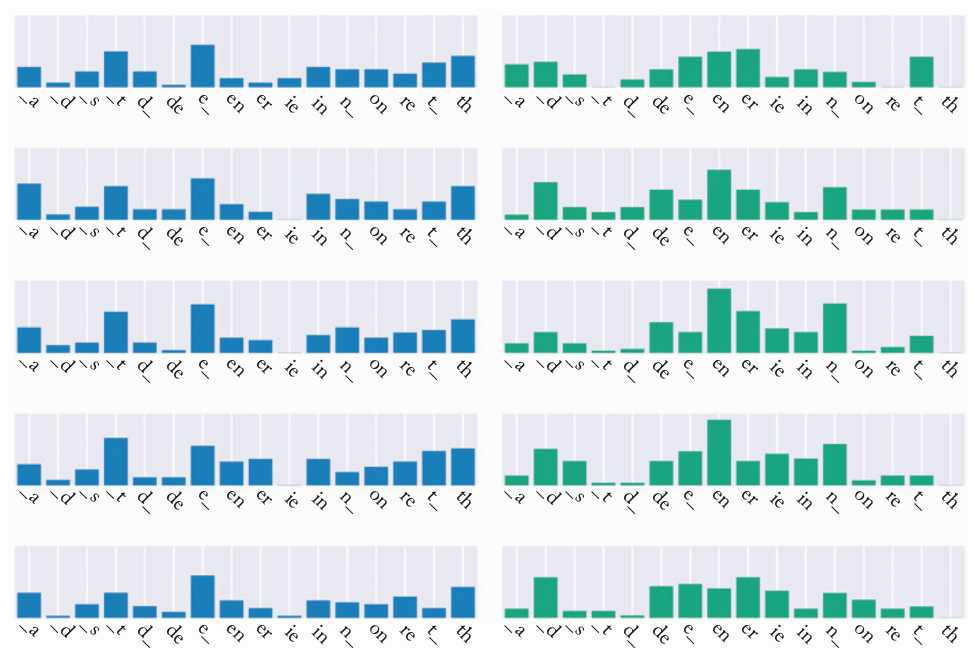
\includegraphics[scale=0.26]{pics/langbigrams.png}
\end{figure}

\scriptsize{Character-bigram histograms for documents in English (left, blue) and German(right,green). Underscores denote spaces. Only the top frequent character-bigrams are showed.}

\footnotetext{Source:\cite{goldberg2017neural}}

\end{frame}


\begin{frame}{Example: Language Detection}
\begin{scriptsize}
\begin{itemize}
\item Previous figure showed clear patterns in the data, and, given a new item, such as:

\begin{figure}[htb]
	\centering
	 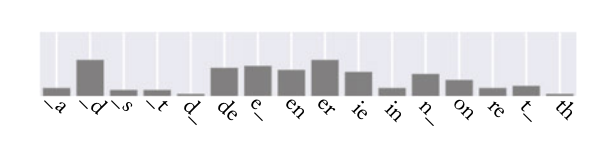
\includegraphics[scale=0.4]{pics/langbigramstest.png}
\end{figure}

\item We could probably tell that it is more similar to the German group than to the English one (observe the frequency of ``th'' and ``ie'').

\item We can't use a single definite rule such as ``if it has th its English'' or ``if it has ie its German''.
\item While German texts have considerably less ``th'' than English, the ``th'' may and does occur in German texts, and similarly the ``ie'' combination does occur in English.


\end{itemize}


\end{scriptsize}
\end{frame}



\begin{frame}{Example: Language Detection}
\begin{scriptsize}
\begin{itemize}
\item The decision requires weighting different factors relative to each other.
\item We can formalize the problem in a machine-learning setup using a linear model:
\begin{equation}
\begin{split}
\hat{y} \quad = sign(f(\vec{x})) & = sign(\vec{x}\cdot \vec{w} + b) \\ 
& = sign(\vec{x}_{aa}\times \vec{w}_{aa}+ \vec{x}_{ab}\times \vec{w}_{ab}+ \vec{x}_{ac}\times \vec{w}_{ac} \dots +b)
\end{split}
\end{equation}
\item A document will be considered English if $f(\vec{x}) \geq 0$  and as German otherwise.
\end{itemize}

\begin{block}{Intuition}
\begin{enumerate}
\item Learning should assign large positive values to $\vec{w}$ entries associated with letter pairs that are much more common in English than in German (i.e., ``th'').
\item It should also assign negative values to letter pairs that are much more common in German than in English (``ie'', ``en'').
\item Finally, it should assign  values around zero to letter pairs that are either common or rare in both languages.
\end{enumerate}
\end{block}
\end{scriptsize}
\end{frame}




\begin{frame}{Log-linear Binary classifcation}
\begin{scriptsize}
\begin{itemize}
\item The output $f(\vec{x})$ is in the range $[-\infty,\infty]$ , and we map it to one of two classes $\{-1,+1\}$ using the $sign$ function.
\item This is a good fit if all we care about is the assigned class.
\item We may be interested also in the confidence of the decision, or the probability that the classifier assigns to the class.
\item An alternative that facilitates this is to map instead to the range $[0,1]$, by pushing the output through a squashing function such as the sigmoid $\sigma(x)$:
\begin{equation}
\sigma(x) = \frac{1}{1+e^{-x}}  
\end{equation}
resulting in: 
\begin{equation}
\hat{y}=\sigma(f(\vec{x})) = \frac{1}{1+e^{-\vec{x}\cdot \vec{w}+b}}  
\end{equation}

\end{itemize}
\end{scriptsize}
\end{frame}


\begin{frame}{The Sigmoid function}
\begin{figure}[htb]
	\centering
	 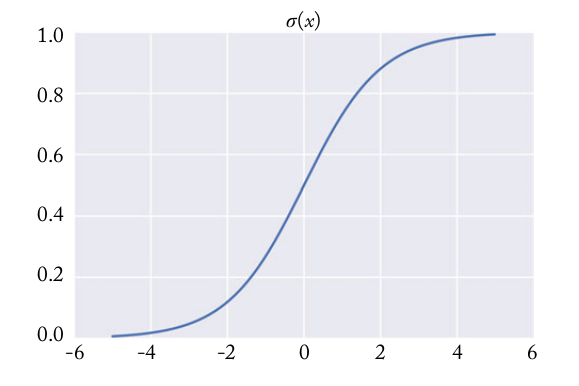
\includegraphics[scale=0.5]{pics/sigmoid.png}
\end{figure}
\end{frame}



\begin{frame}{The Sigmoid function}

\begin{scriptsize}
\begin{itemize}
\item The sigmoid function is is monotonically increasing, and maps values
to the range $[0, 1]$, with $0$ being mapped to $\frac{1}{2}$.
\item When used with a suitable loss function (discussed later) the binary predictions made through the log-linear model can be interpreted as class membership probability estimates:
\begin{equation}
 \sigma(f(\vec{x})) = P(\hat{y} = 1| \vec{x}) \quad \text{of $\vec{x}$ belonging to the positive class.}
\end{equation}
\item We also get $P(\hat{y} = 0| \vec{x}) = 1 - P(\hat{y} = 1| \vec{x}) = 1 -  \sigma(f(\vec{x}))$
\item The closer the value is to $0$ or $1$ the more certain the model is in its class membership prediction, with the value of $0.5$ indicating model uncertainty.
\end{itemize}
\end{scriptsize}
\end{frame}




\begin{frame}{Multi-class Classification}

\begin{scriptsize}
\begin{itemize}
\item Most classification problems are of a multi-class nature: examples are assigned to one of $k$ different classes.
\item Example: we are given a document and asked to classify it into one of six possible languages: English, French, German, Italian, Spanish, Other.
\item Possible solution: consider six weight vectors $\vec{w}_{EN}$,$\vec{w}_{FR},\dots$ and biases (one for each language).
\item Predict the language resulting in the highest score:
\begin{equation}
 \hat{y} = f(\vec{x}) = \operatorname{argmax}_{L \in \{ EN,FR,GR,IT,SP,O \}} \quad \vec{x}\cdot \vec{w}_L+ b_{L}
\end{equation}
\end{itemize}
\end{scriptsize}
\end{frame}



\begin{frame}{Multi-class Classification}

\begin{scriptsize}
\begin{itemize}
\item The six sets of parameters $\vec{w}_L \in  \mathcal{R}^{784}$ and $b_L$  can be arranged as a matrix $W \in \mathcal{R}^{784\times6}$ and vector $\vec{b} \in \mathcal{R}^6$ , and the equation re-written as:
\begin{equation}
 \begin{split}
  \vec{\hat{y}} = f(\vec{x}) = \quad & \vec{x} \cdot W + \vec{b}\\
   \text{prediction} = \hat{y} = \quad  & \operatorname{argmax}_i \vec{\hat{y}}_{[i]} 
 \end{split}
\end{equation}

\item Here $\vec{\hat{y}} \in \mathcal{R}^6$ is a vector of the scores assigned by the model to each language, and we again determine the predicted language by taking the argmax over the entries of $\vec{\hat{y}}$ (the columns with the highest value).

\end{itemize}
\end{scriptsize}
\end{frame}


\begin{frame}{Representations}

\begin{scriptsize}
\begin{itemize}
\item Consider the vector $\vec{\hat{y}}$  resulting from applying a trained model to a document.
\item The vector can be considered as a representation of the document.
\item It captures the properties of the document that are important to us:  the scores of the different languages.
\item The representation $\vec{\hat{y}}$  contains strictly more information than the prediction $\operatorname{argmax}_i \vec{\hat{y}}_{[i]} $.
\item Example: $\vec{\hat{y}}$ can be used to distinguish documents in which the main language is German, but which also contain a sizeable amount of French words.
\item Clustering documents based on $\vec{\hat{y}}$ could help to discover documents written in regional dialects, or by multilingual authors.


\end{itemize}
\end{scriptsize}
\end{frame}


\begin{frame}{Representations}

\begin{scriptsize}
\begin{itemize}
\item The vectors $\vec{x}$ containing the normalized letter-bigram counts for the documents are also representations of the documents.
\item Arguably containing a similar kind of information to the vectors $\vec{\hat{y}}$. 
\item However, the representations in  $\vec{\hat{y}}$ is more compact (6 entries instead of 784) and more specialized for the language prediction objective.
\item Clustering by the vectors $\vec{x}$ would likely reveal document similarities that are not due to a particular mix of languages, but perhaps due to the document's topic or writing styles.
\end{itemize}
\end{scriptsize}
\end{frame}


\begin{frame}{Representations}

\begin{scriptsize}
\begin{itemize}
\item The trained matrix $W \in \mathcal{R}^{784 \times 6}$  can also be considered as containing learned representations.
\item We can consider two views of $W$, as rows or as columns.

\begin{figure}[htb]
	\centering
	 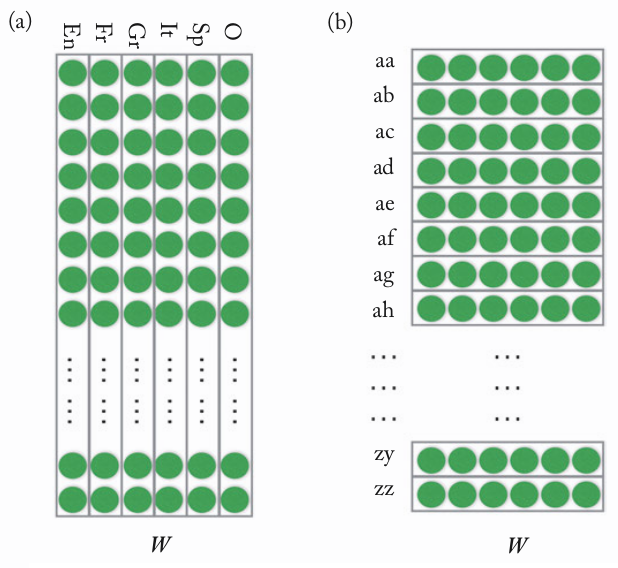
\includegraphics[scale=0.35]{pics/2rep.png}
\end{figure}

Two views of the $W$ matrix. (a) Each column corresponds to a language. (b) Each row
corresponds to a letter bigram. Source: \cite{goldberg2017neural}.


\end{itemize}
\end{scriptsize}
\end{frame}



\begin{frame}{Representations}

\begin{scriptsize}
\begin{itemize}
\item A column of $W$ can be taken to be a $784$-dimensional vector representation of a language in terms of its characteristic letter-bigram patterns.
\item We can then cluster the 6 language vectors according to their similarity.
\item Each of the 784 rows of $W$ provide a 6-dimensional vector representation of that bigram in terms of the languages it prompts.

\end{itemize}
\end{scriptsize}
\end{frame}


\begin{frame}{Representations}

\begin{scriptsize}
\begin{itemize}
\item Representations are central to deep learning.
\item One could argue that the main power of deep-learning is the ability to learn good representations.
\item In the linear case, the representations are interpretable.
\item We can assign a meaningful interpretation to each dimension in the
representation vector.
\item For example: each dimension corresponds to a particular language or letter-bigram.
\end{itemize}
\end{scriptsize}
\end{frame}


\begin{frame}{Representations}

\begin{scriptsize}
\begin{itemize}
\item Deep learning models, on the other hand,  often learn a cascade of representations of the input that build on top of each other. 
\item These representations are often not interpretable.
\item We do not know which properties of the input they capture.
\item However, they are still very useful for making predictions.
\end{itemize}
\end{scriptsize}
\end{frame}

\begin{frame}{One-Hot Vector Representation}

\begin{scriptsize}
\begin{itemize}
\item The input vector $\vec{x}$ in our language classification example contains the normalized bigram counts in the document $D$.
\item This vector can be decomposed into an average of $|D|$ vectors, each corresponding to a particular document position $i$:
\begin{equation}
 \vec{x} = \frac{1}{|D|} \sum_{i=1}^{|D|} \vec{x}^{D_{[i]}}
\end{equation}
\item Here, $D_{[i]}$ is the bigram at document position $i$.
\item Each vector  $\vec{x}^{D_{[i]}} \in \mathcal{R}^{784}$ is a one-hot vector.
\end{itemize}
\end{scriptsize}
\end{frame}

\begin{frame}{One-Hot Vector Representation}

\begin{scriptsize}
\begin{itemize}
\item A one-hot vector: all entries are zero except the single entry corresponding to the letter bigram $D_{[i]}$, which is 1.
\item The resulting vector $\vec{x}$ is commonly referred to as an averaged bag of bigrams (more generally averaged bag of words , or just bag of words).
\item Bag-of-words (BOW) representations contain information about the identities of all the ``words'' (here, bigrams) of the document, without considering their order.
\item A one-hot representation can be considered as a bag-of-a-single-word.
\end{itemize}
\end{scriptsize}
\end{frame}



\begin{frame}{One-Hot Vector Representation}

\begin{scriptsize}

\begin{figure}[htb]
	\centering
	 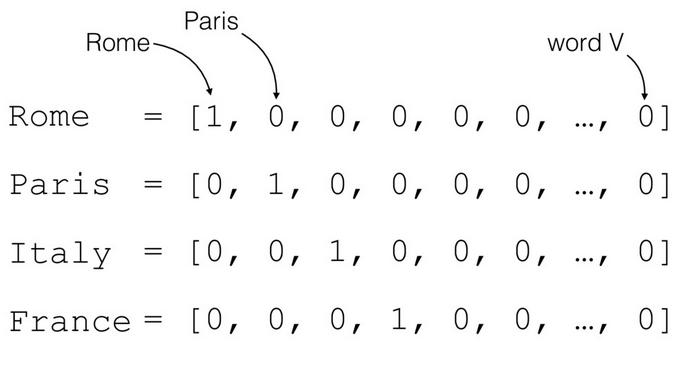
\includegraphics[scale=0.35]{pics/onehot.png}
\end{figure}

One-hot vectors of words. Source: \url{https://medium.com/@athif.shaffy/one-hot-encoding-of-text-b69124bef0a7}.

\end{scriptsize}
\end{frame}


\begin{frame}{Log-linear Multi-class Classification}

\begin{scriptsize}
\begin{itemize}
\item In the binary case, we transformed the linear prediction into a probability estimate by passing it through the sigmoid function, resulting in a log-linear model.
\item The analog for the multi-class case is passing the score vector through the \textbf{softmax} function:
\begin{equation}
 \operatorname{softmax}(\vec{x})_{[i]} = \frac{e^{\vec{x}_{[i]}}}{\sum_j e^{\vec{x}_{[j]}}}
\end{equation}
Resulting in:
\begin{equation}
\begin{split}
\vec{\hat{y}} \quad & =  \operatorname{softmax}(\vec{x} \cdot W + \vec{b})  \\
\vec{\hat{y}}_{[i]} \quad & = \frac{e^{(\vec{x} \cdot W + \vec{b})_{[i]}}}{\sum_j e^{(\vec{x} \cdot W + \vec{b})_{[j]}}}
\end{split}
\end{equation}
\item The softmax transformation forces the values in $\hat{\vec{y}}$ to be positive and sum to 1, making them interpretable as a probability distribution.
\end{itemize}
\end{scriptsize}
\end{frame}





\begin{frame}{Training}
\begin{scriptsize}
\begin{itemize}
\item  When training a parameterized function (e.g., a linear model, a neural network) one defines a loss function $L(\hat{y}, y)$, stating the loss of predicting $\hat{y}$ when the true output is y.

\begin{displaymath}
L(f(\vec{x};\Theta), y) 
\end{displaymath}

\item We use the symbol $\Theta$ to denote all the parameters of the model (e.g.,  $W, \vec{b}$)

\item The training objective is then to minimize the loss across the different training examples. 


\item Formally, a loss function $L(\hat{y},y)$ assigns a numerical score (a scalar) to a predicted output $\hat{y}$ given the true expected output $y$. 

\end{itemize}
\end{scriptsize}
\end{frame}



\begin{frame}{Training}
\begin{scriptsize}
\begin{itemize}
\item The loss function should attain its minimum value for cases where the prediction is correct.

\item We can also define a corpus-wide loss with respect to the parameters $\Theta$ as the average loss over all training examples:

\begin{displaymath}
 \mathcal{L}(\Theta) = \frac{1}{n} \sum_{i=1}^n L(f(\vec{x}_i;\Theta), y_i)
\end{displaymath}

\item The goal of the training algorithm is then to set the values of the parameters $\Theta$  such that the value of $\mathcal{L}$ is minimized.


\begin{displaymath}
 \hat{\Theta} = \operatorname{argmin}_{\Theta} \mathcal{L}(\Theta) =  \operatorname{argmin}_{\Theta} \frac{1}{n} \sum_{i=1}^n L(f(\vec{x}_i;\Theta), y_i)
\end{displaymath}


\end{itemize}


\end{scriptsize}
\end{frame}



\begin{frame}{Gradient-based Optimization}
\begin{scriptsize}
\begin{itemize}
\item Functions are trained using  gradient-based methods.

\item They work by repeatedly computing an estimate of the loss $L$ over the training set.



\item The training method computes gradients of the parameters ($\Theta$)  with respect to the loss estimate, and moving the parameters in the opposite directions of the gradient. 

\item Different optimization methods differ in how the error estimate is computed, and how moving in the opposite direction of the gradient is defined.

\item If the function is convex, the optimum will be a global one.

\item Otherwise, the process is only guaranteed to find a local optimum.


\end{itemize}


\end{scriptsize}
\end{frame}


\begin{frame}{Gradient Descent}
\begin{figure}[htb]
	\centering
	 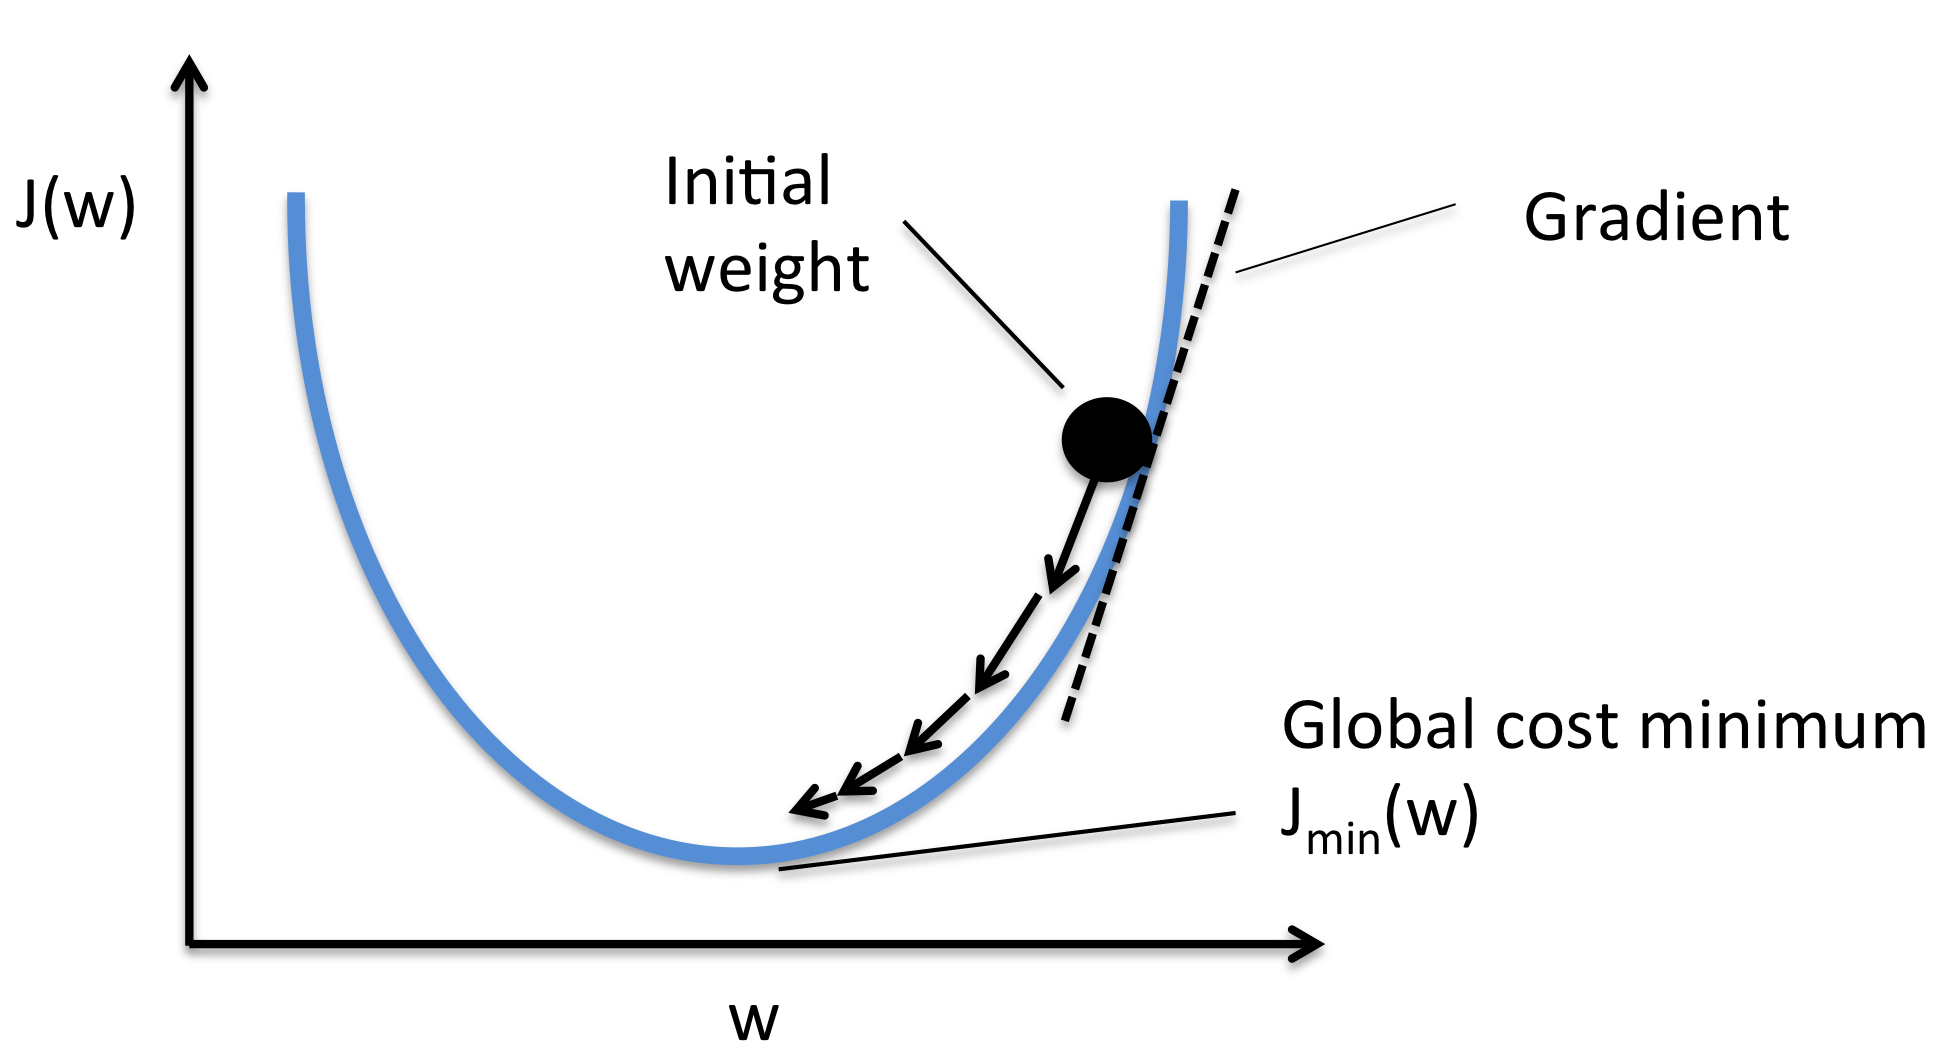
\includegraphics[scale=0.15]{pics/sgd.png}
\end{figure}

\footnotetext{Source: \url{https://sebastianraschka.com/images/faq/closed-form-vs-gd/ball.png}}

\end{frame}


\begin{frame}{Gradient Descent}
\begin{figure}[htb]
	\centering
	 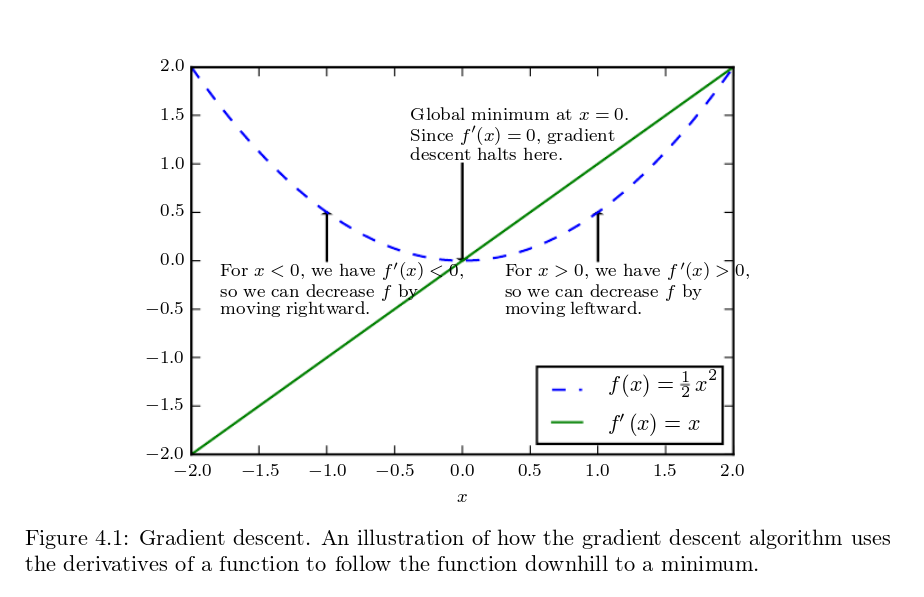
\includegraphics[scale=0.45]{pics/gradientdescent.png}
\end{figure}

\footnotetext{\cite{goodfellow2016deep}}

\end{frame}



\begin{frame}{Online Stochastic Gradient Descent}

\begin{scriptsize}
\begin{itemize}
\item All the parameters are initialized with random values ($\Theta$).
\item For each training example $(x,y)$ we calculate the loss $L$ with current values of $\Theta$.
\item Then we update the parameters with the following rule until convergence:
\item $\Theta_i \leftarrow \Theta_i - \eta \frac{\partial L}{\Theta_i}(\hat{y},y)$  (for all parameters $\Theta_i$)

\begin{figure}[htb]
	\centering
	 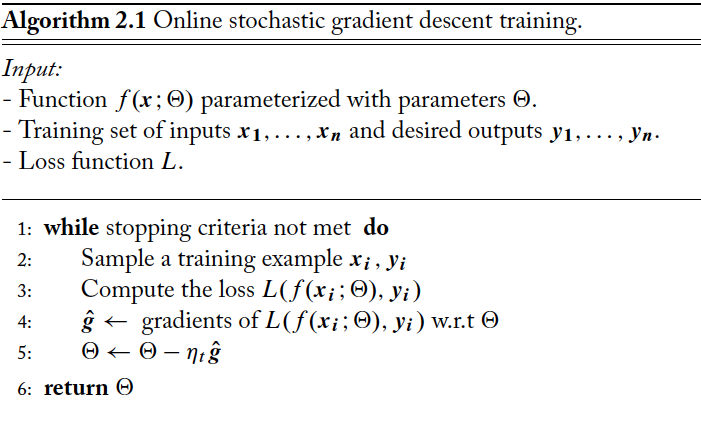
\includegraphics[scale=0.3]{pics/Online-SGD.png}
\end{figure}

\end{itemize}


\footnotetext{Source:\cite{goldberg2017neural}}

\end{scriptsize}


\end{frame}



\begin{frame}{Online Stochastic Gradient Descent}


\begin{scriptsize}
\begin{itemize}
\item The learning rate can either be fixed throughout the
training process, or decay as a function of the time step $t$.
\item  The error calculated in line 3 is based on a single training example, and is thus just a rough estimate of the corpus-wide loss $L$ that we are aiming to minimize. 
\item The noise in the loss computation may result in inaccurate gradients (single examples may provide noisy information).

\end{itemize}


\end{scriptsize}

\end{frame}






\begin{frame}{Mini-batch Stochastic Gradient Descent}

\begin{scriptsize}
\begin{itemize}
\item A common way of reducing this noise is
to estimate the error and the gradients based on a sample of $m$ examples.
\item This gives rise to the minibatch SGD algorithm




\begin{figure}[htb]
	\centering
	 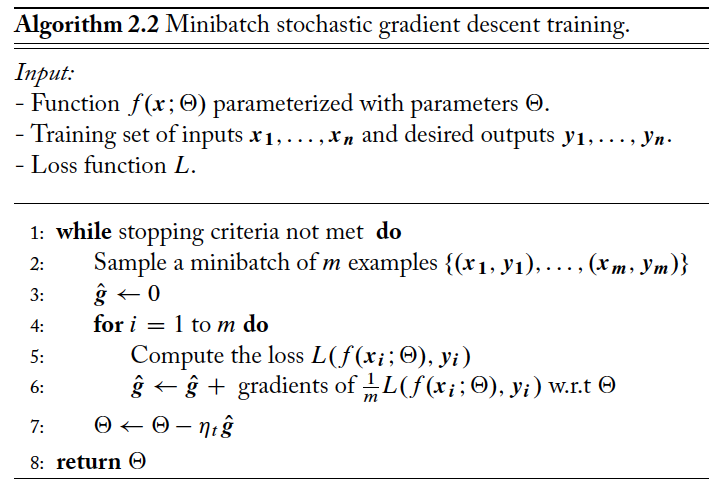
\includegraphics[scale=0.25]{pics/minibatch-SGD.png}
\end{figure}

\item Higher values of $m$ provide better estimates of the corpus-wide gradients, while smaller values allow more updates and in turn faster convergence.

\item For modest sizes of $m$ , some computing architectures (i.e., GPUs) allow an efficient parallel implementation of the computation in lines 3-6.

\end{itemize}
\end{scriptsize}

\footnotetext{Source:\cite{goldberg2017neural}}

\end{frame}



\begin{frame}{Loss Functions}
\begin{scriptsize}
\begin{itemize}
 \item Hinge (or SVM loss):  for binary classification problems, the classifier's output is a single scalar $\tilde{y}$ and the intended output y is in $\{+1,-1\}$.  The classification rule is $\hat{y} = sign(\tilde{y})$, and a classification is considered correct if $y \cdot \tilde{y} > 0$.  
 \begin{displaymath}
  L_{\text{hinge}(\text{binary})}(\tilde{y},y) = \max(0,1-y \cdot \tilde{y})  
 \end{displaymath}

 \item Binary cross entropy (or logistic loss): is used in binary classification with conditional probability outputs. The classifier's output $\tilde{y}$ is transformed using the sigmoid function to the range $[0,1]$ , and is interpreted as the conditional probability $P(y=1|x)$.
  \begin{displaymath}
  L_{\text{logistic}}(\hat{y},y) = -y \log \hat{y} - (1-y) \log(1-\hat{y})  
 \end{displaymath}
 
\end{itemize}
\end{scriptsize}

\end{frame}


\begin{frame}{Loss Functions}
\begin{scriptsize}
\begin{itemize}

%\hat{y}=\sigma(f(\vec{x})) = \frac{1}{1+e^{-\vec{x}\cdot \vec{w}+b}} 

 \item The logistic loss has a probalistic interpration:
 \item We assume that $P(y =1 | \vec{x} ; \Theta) = \sigma(f(\vec{x})) = \frac{1}{1+e^{-\vec{x}\cdot \vec{w}+b}}$  and $P(y = 0 | \vec{x} ; \Theta) = 1 - \sigma(f(\vec{x}))$
 \item We can write this is a more compact way: 
 \begin{displaymath}
  P(y | \vec{x} ; \Theta) = \sigma(f(\vec{x}))^y\times(1-\sigma(f(\vec{x})))^{1-y}
 \end{displaymath}

 \item The above expression is the probability mass function of the Bernoulli distribution.
 
\item Now we replace $\sigma(f(\vec{x}))$ by $\hat{y}$:
 \begin{displaymath}
  P(y | \vec{x} ; \Theta) = \hat{y}^y\times(1-\hat{y})^{1-y}
 \end{displaymath} 
\item If we perform maximum likelihood estimation to this expression we would apply a logarithm function and maximize the parameters $\Theta$:
 \begin{displaymath}
  y \log \hat{y} + (1-y) \log(1-\hat{y}) 
 \end{displaymath} 
 
\item Maximizing this expression is equivalent to miniziming the logistic loss!
 
\item Many loss functions correspond to the negative log-likelihood of probalistic models!
 
\end{itemize}
\end{scriptsize}

\end{frame}



\begin{frame}{Loss Functions}
\begin{scriptsize}
\begin{itemize}

 \item Categorical cross-entropy loss:  is used when a probabilistic interpretation of multi-class scores is desired. It measures the dissimilarity between the true label distribution $\vec{y}$ and the predicted label distribution $\vec{\hat{y}}$. 
   \begin{displaymath}
  L_{\text{cross-entropy}}(\vec{\hat{y}},\vec{y}) = - \sum_{i} \vec{y}_{[i]} \log(\vec{\hat{y}}_{[i]})   
 \end{displaymath}
 \item When using the cross-entropy loss, it is assumed that the classifier's output is transformed using the softmax transformation.

 \item The softmax function squashes the $k$-dimensional output to values in the range (0,1) with all entries adding up to 1. Hence, $\vec{\hat{y}}_{[i]} = P( y = i |x)$ represent the class membership conditional distribution.
 
\end{itemize}
\end{scriptsize}


\end{frame}


\begin{frame}{Loss Functions}
\begin{scriptsize}
\begin{itemize}



\item For hard-classification problems in which each training example has a single correct class assignment, $\vec{y}$ is a one-hot vector representing the true class. 
\item In such cases, the cross entropy can be simplified to:
   \begin{displaymath}
  L_{\text{cross-entropy(hard classification)}}(\vec{\hat{y}},\vec{y}) = -\log(\vec{\hat{y}}_{[t]})   
 \end{displaymath}
 where $t$ is the correct class assignment.



 
\end{itemize}
\end{scriptsize}


\end{frame}


\begin{frame}{Regularization}
\begin{scriptsize}
\begin{itemize}
 \item Our optimization problem may admit multiple solutions, and, especially in higher dimensions, it can also over-fit.
 \item Scenario: In our language identification problem one of the documents in the training set ($\vec{x}_O$) is an outlier.
 \item The document is actually in German, but is labeled as French.
 
 \item In order to drive the loss down, the learner can identify features (letter bigrams) in $\vec{x}_O$ that occur in only few other documents.
 
 \item The learner will give these features very strong weights toward the (incorrect) French class. 

\end{itemize}
\end{scriptsize}

\end{frame}


\begin{frame}{Regularization}
\begin{scriptsize}
\begin{itemize}
  \item This is a bad solution to the learning problem.
 \item The model is learning something incorrect.
 \item Test German documents which share many words with $\vec{x}_O$ could be mistakenly classified as French. 
 \item We would like to control for such cases by driving the learner away from such misguided solutions.
 \item Idea: it is OK to mis-classify a few examples if they don't fit well with the rest.
 
\end{itemize}
\end{scriptsize}

\end{frame}



\begin{frame}{Regularization}
\begin{scriptsize}
\begin{itemize}
  \item Regularization: we add a regularization term $R$ to the optimization objective.
  \item  The goal of this term: to control the complexity (large weights) of the parameter value ($\Theta$), and avoid cases of overfitting:
\begin{equation}
 \begin{split}
  \hat{\Theta} \quad & =  \operatorname{argmin}_{\Theta} \mathcal{L}(\Theta) + \lambda R(\Theta) \\
     \quad & =  \operatorname{argmin}_{\Theta} \frac{1}{n} \sum_{i=1}^n L(f(\vec{x}_i;\Theta), y_i) + \lambda R(\Theta) \\
 \end{split}
\end{equation}  
\item The regularization term considers the parameter values, and scores their complexity.  
\item The value of hyperparameter $\lambda$ has to be set manually, based on the classification performance on a development set.   
 
\end{itemize}
\end{scriptsize}

\end{frame}



\begin{frame}{Regularization}
\begin{scriptsize}
\begin{itemize}
  \item  In practice, the regularizers $R$ equate complexity with large weights.
  \item They work to keep the parameter values ($\Theta$) low.
  \item They drive the learner toward solutions with low norms of the parameter matrices ($W$).
  \item Common choices for $R$ are the $L_2$ norm, the $L_1$ norm, and the elastic-net.
\end{itemize}
\end{scriptsize}

\end{frame}


\begin{frame}{L$_2$ Regularization}
\begin{scriptsize}
\begin{itemize}
\item  In $L_2$ regularization, $R$ takes the form of the squared $L_2$ norm of the parameters.
\item Goal: try to keep the sum of the squares of the parameter values low.
  \begin{displaymath}
   R_{L_{2}}(W) = ||W||^{2}_{2} = \sum_{i,j}(W_{[i,l]})^2
  \end{displaymath}
\item The $L_2$ regularizer is also called a gaussian prior or weight decay.
\item $L_2$ regularized models are severely punished for high parameter weights.
\item Once the value is close enough to zero, their effect becomes negligible.
\item The model will prefer to decrease the value of one parameter with high weight by 1 than to decrease the value of ten parameters that already have relatively low weights by 0.1 each.
\end{itemize}
\end{scriptsize}

\end{frame}



\begin{frame}{L$_1$ Regularization}
\begin{scriptsize}
\begin{itemize}
  \item  In $L_1$ regularization, $R$ takes the form of the $L_1$ norm of the parameters.
  \item Goal: try to keep the sum of the absolute values of the parameters low.
  \begin{displaymath}
   R_{L_{1}}(W) = ||W||_{1} = \sum_{i,j} |W_{[i,l]}|
  \end{displaymath}
 \item In contrast to $L_2$ , the $L_1$ regularizer is punished uniformly for low and high values.
 \item It has an incentive to decrease all the non-zero parameter values toward zero. 
 \item It thus encourages a sparse solutions—models with many parameters with a zero value. 
 \item The $L_1$ regularizer is also called a sparse prior or lasso \cite{tibshirani1996regression}. 
  \end{itemize}
\end{scriptsize}

\end{frame}


\begin{frame}{Elastic-Net}
\begin{scriptsize}
\begin{itemize}
  \item  The elastic-net regularization \cite{zou2005regularization} combines both $L_1$ and $L_2$ regularization:
 
 \begin{displaymath}
  R_{\text{elactic-net}}(W) = \lambda_{1}R_{L_{1}}(W) + \lambda_{2}R_{L_{2}}(W)
 \end{displaymath}

  
\end{itemize}
\end{scriptsize}

\end{frame}



\begin{frame}{Beyond SGD}
\begin{scriptsize}
\begin{itemize}

 \item While the SGD algorithm can and often does produce good results, more advanced algorithms are also available. 
 \item The SGD+Momentum \cite{polyak1964some} and Nesterov Momentum \cite{nesterov2018lectures,sutskever2013importance}  algorithms are variants of SGD in which previous gradients are accumulated and affect the current update. 
\item Adaptive learning rate algorithms including AdaGrad \cite{duchi2011adaptive}, AdaDelta \cite{zeiler2012adadelta}, RMSProp \cite{tieleman2012lecture}, and Adam \cite{kingma2014adam} are designed to select the learning rate for each minibatch.
\item This sometimes done on a per-coordinate basis, potentially alleviating the need of fiddling with learning rate scheduling. 
\item For details of these algorithms, see the original papers or \cite{goodfellow2016deep}(Sections 8.3, 8.4).
 
\end{itemize}
\end{scriptsize}

\end{frame}




\begin{frame}{Train, Test, and Validation Sets}
\begin{scriptsize}
\begin{itemize}
\item When training a model our goal is to produce a function $f(\vec{x})$ that correctly maps inputs $\vec{x}$ to outputs $\hat{y}$ as evidenced by the training set.
\item Performance on training data can be misleading: our goal is to train a function capable of generalizing to unseen examples.  
\item Held-out set: split training set into training and testing subsets (80\% and 20\% splits). Train on training and compute accuracy on testing.
\item Problem: in practice you often train several models, compare their quality, and select the best one. 
\item Selecting the best model according to the held-out set's accuracy will result in an overly optimistic estimate of the model's quality.
\item You don't know if the chosen settings of the final classifier are good in general, or are just good for the particular examples in the held-out sets.

\end{itemize}
\end{scriptsize}
\end{frame}


\begin{frame}{Train, Test, and Validation Sets}
\begin{scriptsize}
\begin{itemize}
\item The accepted methodology is to use a three-way split of the data into train, validation (also called development), and test sets\footnote{An alternative approach is cross-validation, but it doesn't scale well for training deep neural networks.}. 
\item This gives you two held-out sets: a validation set (also called development set ), and a test set.
\item All the experiments, tweaks, error analysis, and model selection should be performed based on the validation set. 
\item Then, a single run of the final model over the test set will give a good estimate of its expected quality on unseen examples. 
\item It is important to keep the test set as pristine as possible, running as few experiments as possible on it. 
\item Some even advocate that you should not even look at the examples in the test
set, so as to not bias the way you design your model.



\end{itemize}

\end{scriptsize}
\end{frame}



\begin{frame}{Train, Test, and Validation Sets}
\begin{scriptsize}

 \begin{figure}[htb]
	\centering
	 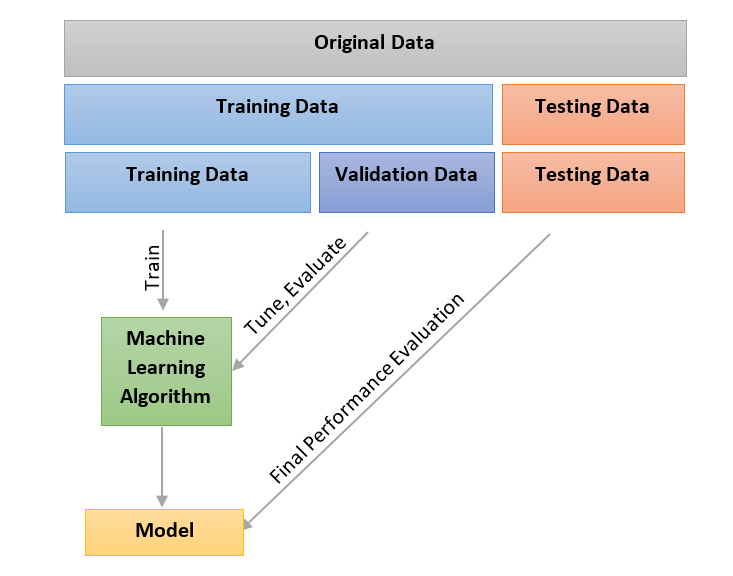
\includegraphics[scale=0.55]{pics/validation.png}
\end{figure}

\footnotetext{source: \url{https://www.codeproject.com/KB/AI/1146582/validation.PNG}}

\end{scriptsize}
\end{frame}


\begin{frame}{A limitation of linear models: the XOR problem}
\begin{scriptsize}
\begin{itemize}
\item The hypothesis class of linear (and log-linear) models is severely restricted.
\item For example, it cannot represent the XOR function, defined as:
\begin{equation}
 \begin{split}
  \operatorname{xor}(0,0) \quad & = 0 \\
  \operatorname{xor}(1,0) \quad & = 1 \\
  \operatorname{xor}(0,1) \quad & = 1 \\
  \operatorname{xor}(1,1) \quad & = 0 \\
 \end{split}
\end{equation}
\end{itemize}
\end{scriptsize}
\end{frame}


\begin{frame}{A limitation of linear models: the XOR problem}
\begin{scriptsize}
\begin{itemize}
\item There is no parameterization $\vec{w} \in \mathcal{R}^2, b \in \mathcal{R}$ such that:
\begin{equation}
 \begin{split}
  (0,0) \cdot \vec{w} +b \quad & < 0 \\
  (0,1) \cdot \vec{w} +b \quad & \geq 0 \\
  (1,0) \cdot \vec{w} +b \quad & \geq 0 \\
  (1,1) \cdot \vec{w} +b \quad & < 0 \\
 \end{split}
\end{equation}
\end{itemize}
\end{scriptsize}
\end{frame}



\begin{frame}{A limitation of linear models: the XOR problem}
\begin{scriptsize}
\begin{itemize}
\item To see why, consider the following plot of the XOR function, where blue Os denote the positive class and green Xs the negative class.
\begin{figure}[htb]
	\centering
	 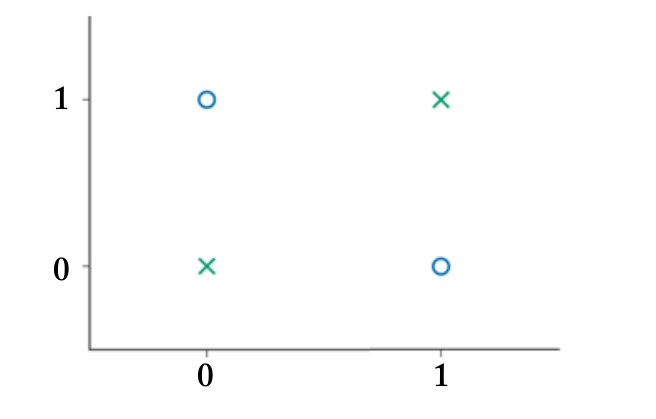
\includegraphics[scale=0.35]{pics/xor.png}
\end{figure}
\item It is clear that no straight line can separate the two classes.
\end{itemize}
\end{scriptsize}
\end{frame}




\begin{frame}{Nonlinear input transformations}
\begin{scriptsize}
\begin{itemize}
\item If we transform the points by feeding each of them through the nonlinear function $\phi(x_1,x_2) = [x_1 \times x_2, x_1 + x_2 ]$ , the XOR problem becomes linearly separable.
\begin{figure}[htb]
	\centering
	 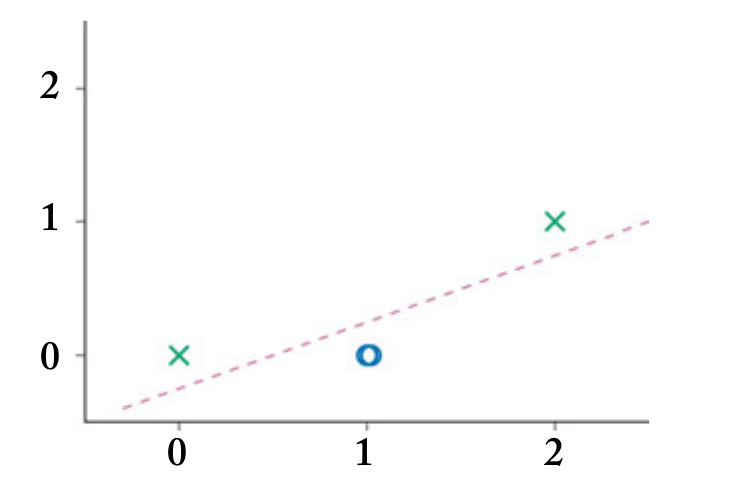
\includegraphics[scale=0.25]{pics/xor2.png}
\end{figure}

\item The function $\phi$ mapped the data into a representation that is suitable for linear classification.

\end{itemize}
\end{scriptsize}
\end{frame}


\begin{frame}{Nonlinear input transformations}
\begin{scriptsize}
\begin{itemize}
\item We can now easily train a linear classifier to solve the XOR problem.
\begin{equation}
 \hat{y} = f(\vec{x}) = \phi(\vec{x}) \cdot \vec{w} +b
\end{equation}
\item Problem: we need to manually define the function $\phi$.
\item This process is dependent on the particular dataset, and requires a lot of human intuition.
\item Solution: define a trainable nonlinear mapping function, and train it in con-
junction with the linear classifier.
\item Finding the suitable representation becomes the responsibility of the training algorithm.
\end{itemize}
\end{scriptsize}
\end{frame}


\begin{frame}{Trainable mapping functions}
\begin{scriptsize}
\begin{itemize}
\item The mapping function can take the form of a parameterized linear model.
\item Followed by a nonlinear activation function $g$ that is applied to each of the output dimensions:
\begin{equation}
\begin{split}
\hat{y} = f(\vec{x}) = \phi(\vec{x}) \cdot \vec{w} +b \\
\phi(\vec{x}) = g(\vec{x}W'+ \vec{b}') \\
\end{split} 
\end{equation}
\end{itemize}
\end{scriptsize}
\end{frame}



\begin{frame}{Trainable mapping functions}
\begin{scriptsize}
\begin{itemize}
\item By taking $g(x) = \operatorname{max}(0, x)$ and $W' = \begin{pmatrix}
    1 & 1 \\ 1 & 1 \end{pmatrix}$, $\vec{b}' = \begin{pmatrix}
    -1 & 0 \end{pmatrix}$.
\item We get an equivalent mapping to $[x_1 \times x_2, x_1 + x_2]$  for the our points of interest (0,0), (0,1), (1,0), and (1,1).
\item This successfuly solves the XOR problem!
\item Learning both the representation function and the linear classifier on top of it at the same time is the main idea behind deep learning and neural networks.
\item In fact, previous equation describes a very common neural network architecture called a multi-layer perceptron (MLP).
\end{itemize}
\end{scriptsize}
\end{frame}




\begin{frame}
\frametitle{Questions?}
%\vspace{1.5cm}
\begin{center}\LARGE Thanks for your Attention!\\ \end{center}



\end{frame}

\begin{frame}[allowframebreaks]\scriptsize
\frametitle{References}
\bibliography{bio}
\bibliographystyle{apalike}
%\bibliographystyle{flexbib}
\end{frame}  


%%%%%%%%%%%%%%%%%%%%%%%%%%%

\end{document}
